\subsection{《共同的底线》}
秦晖这本书写于90年代到2005年左右,出版时是2013年,到现在已经有20年了,但对事实的判断皆为真知灼见,读之获益颇多。

\subsubsection{关于主义}
主义满天飞,但秦晖的这张图把各种思想和主义的源流清晰地表达出来: 
\begin{figure}[htpb]
\centering
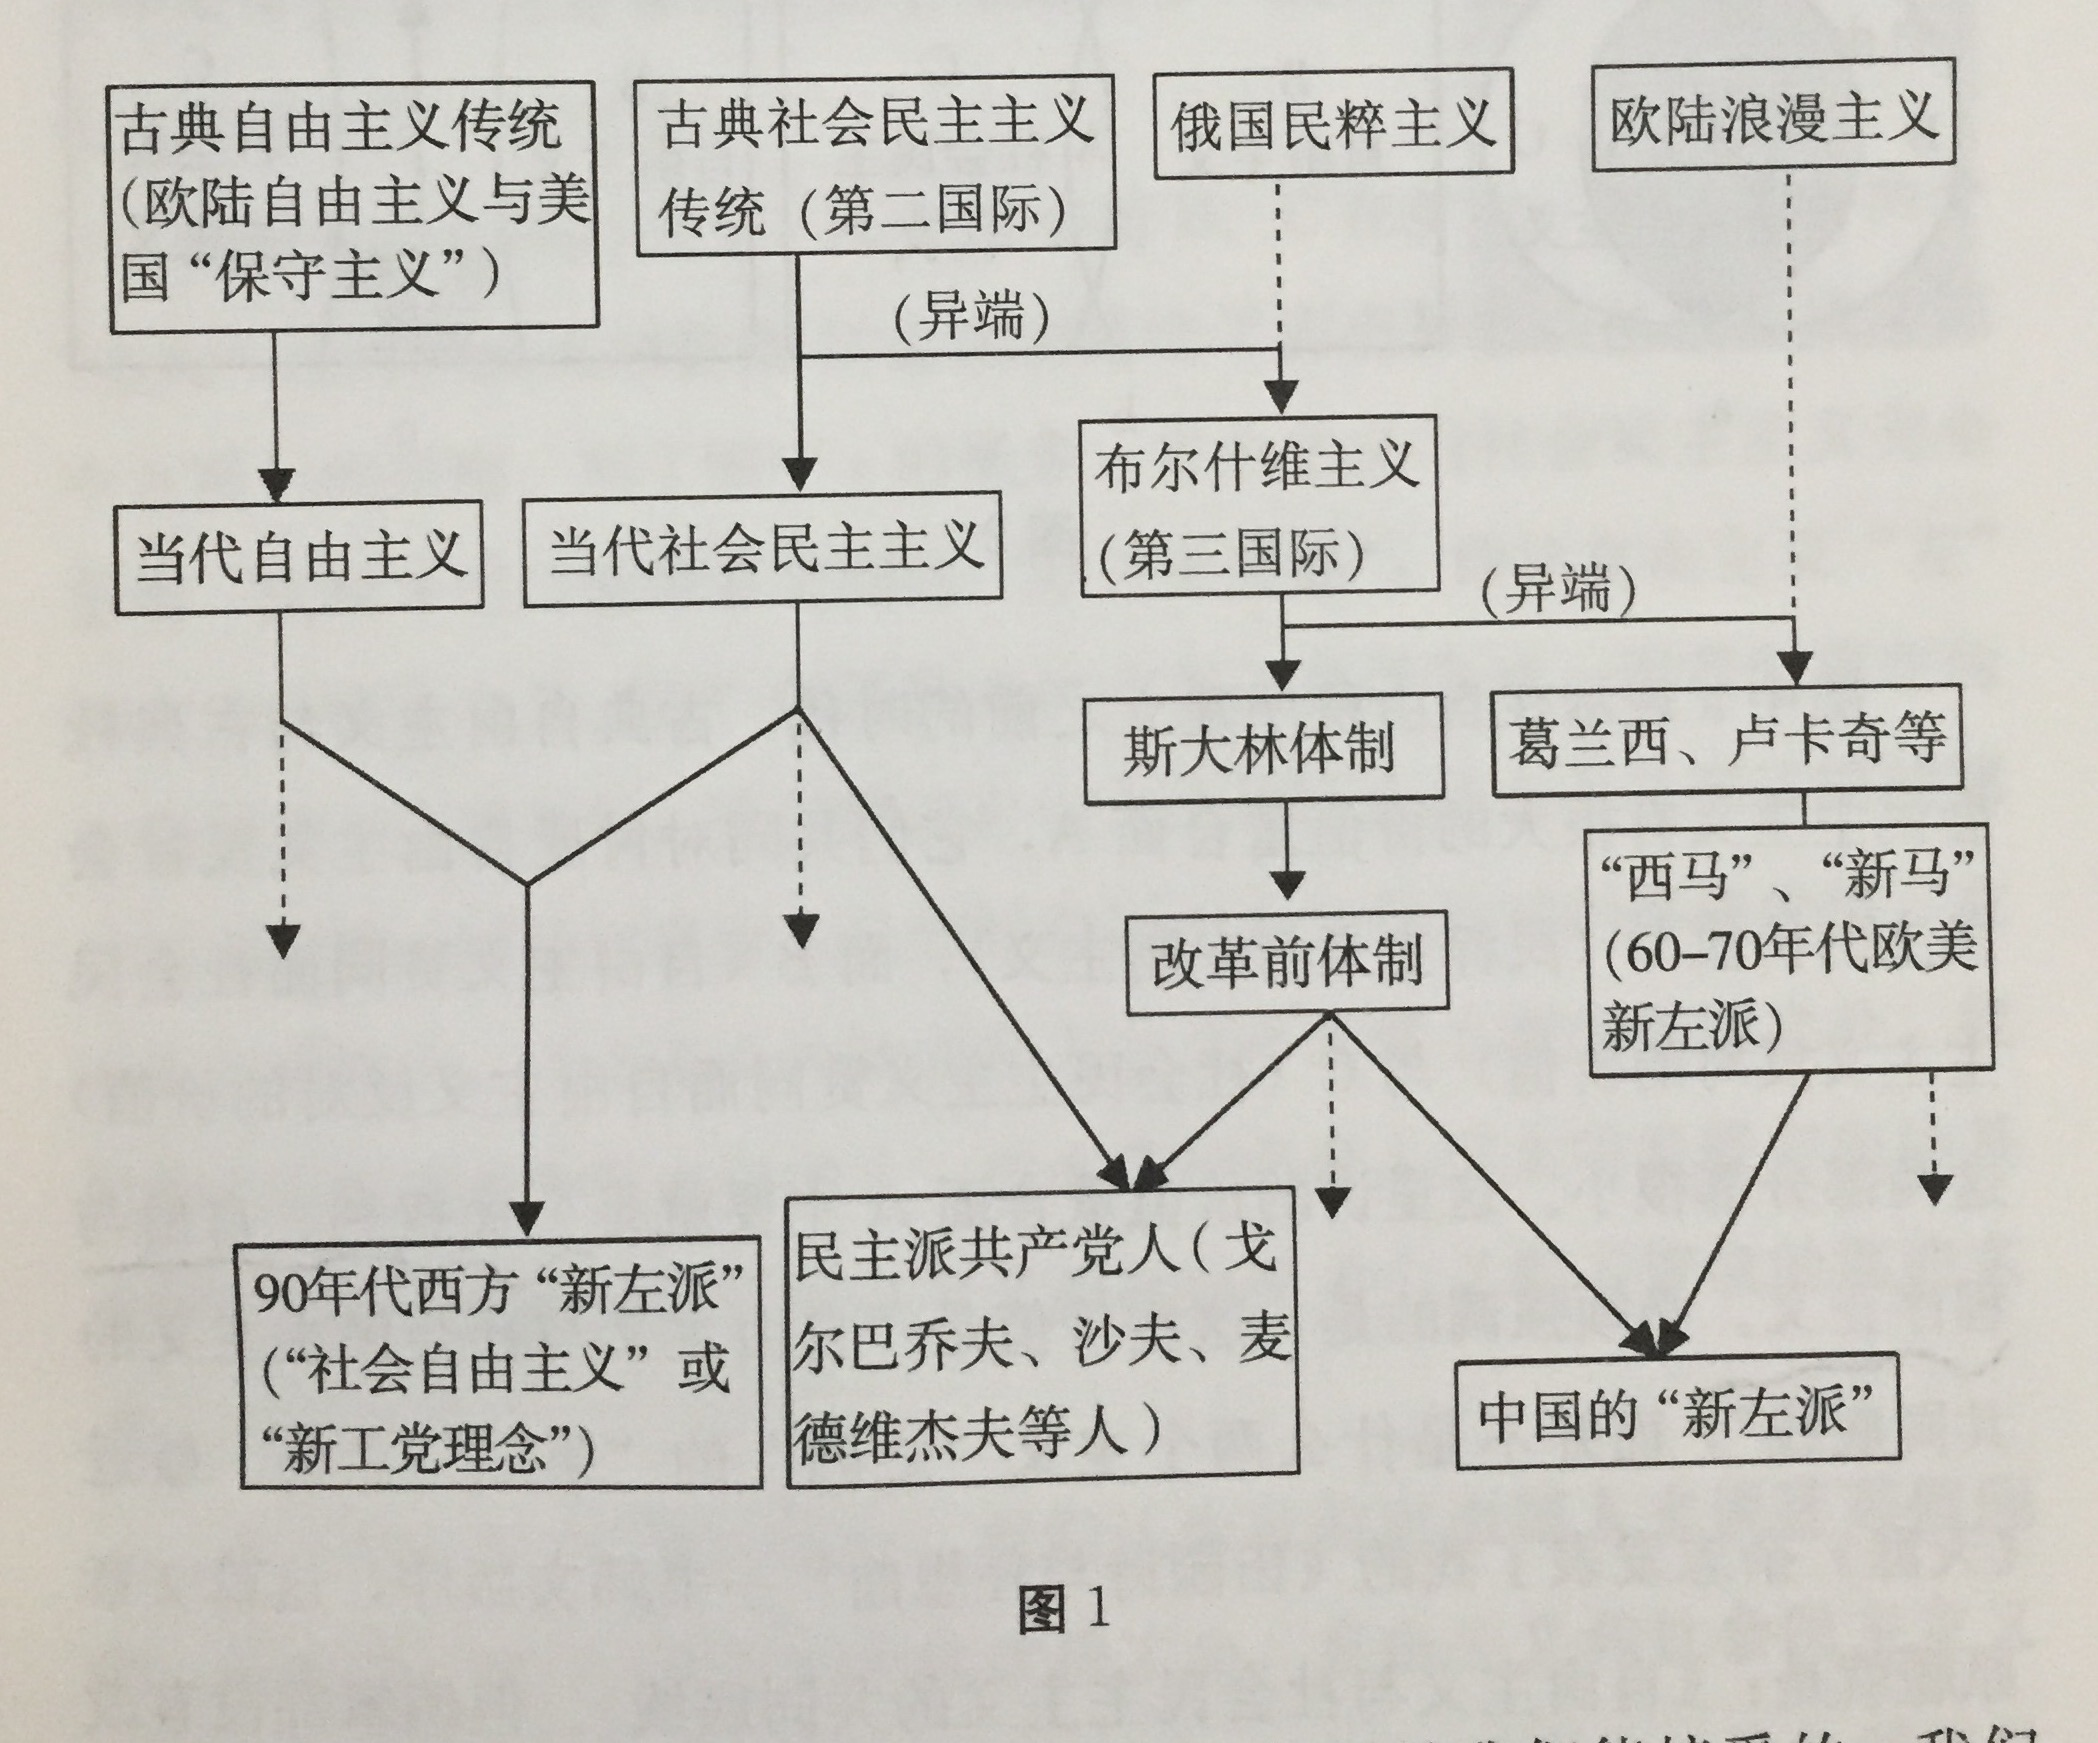
\includegraphics[width=0.5\linewidth]{images/zhuyi.jpg}
\end{figure}
以及
\begin{figure}[htpb]
\centering
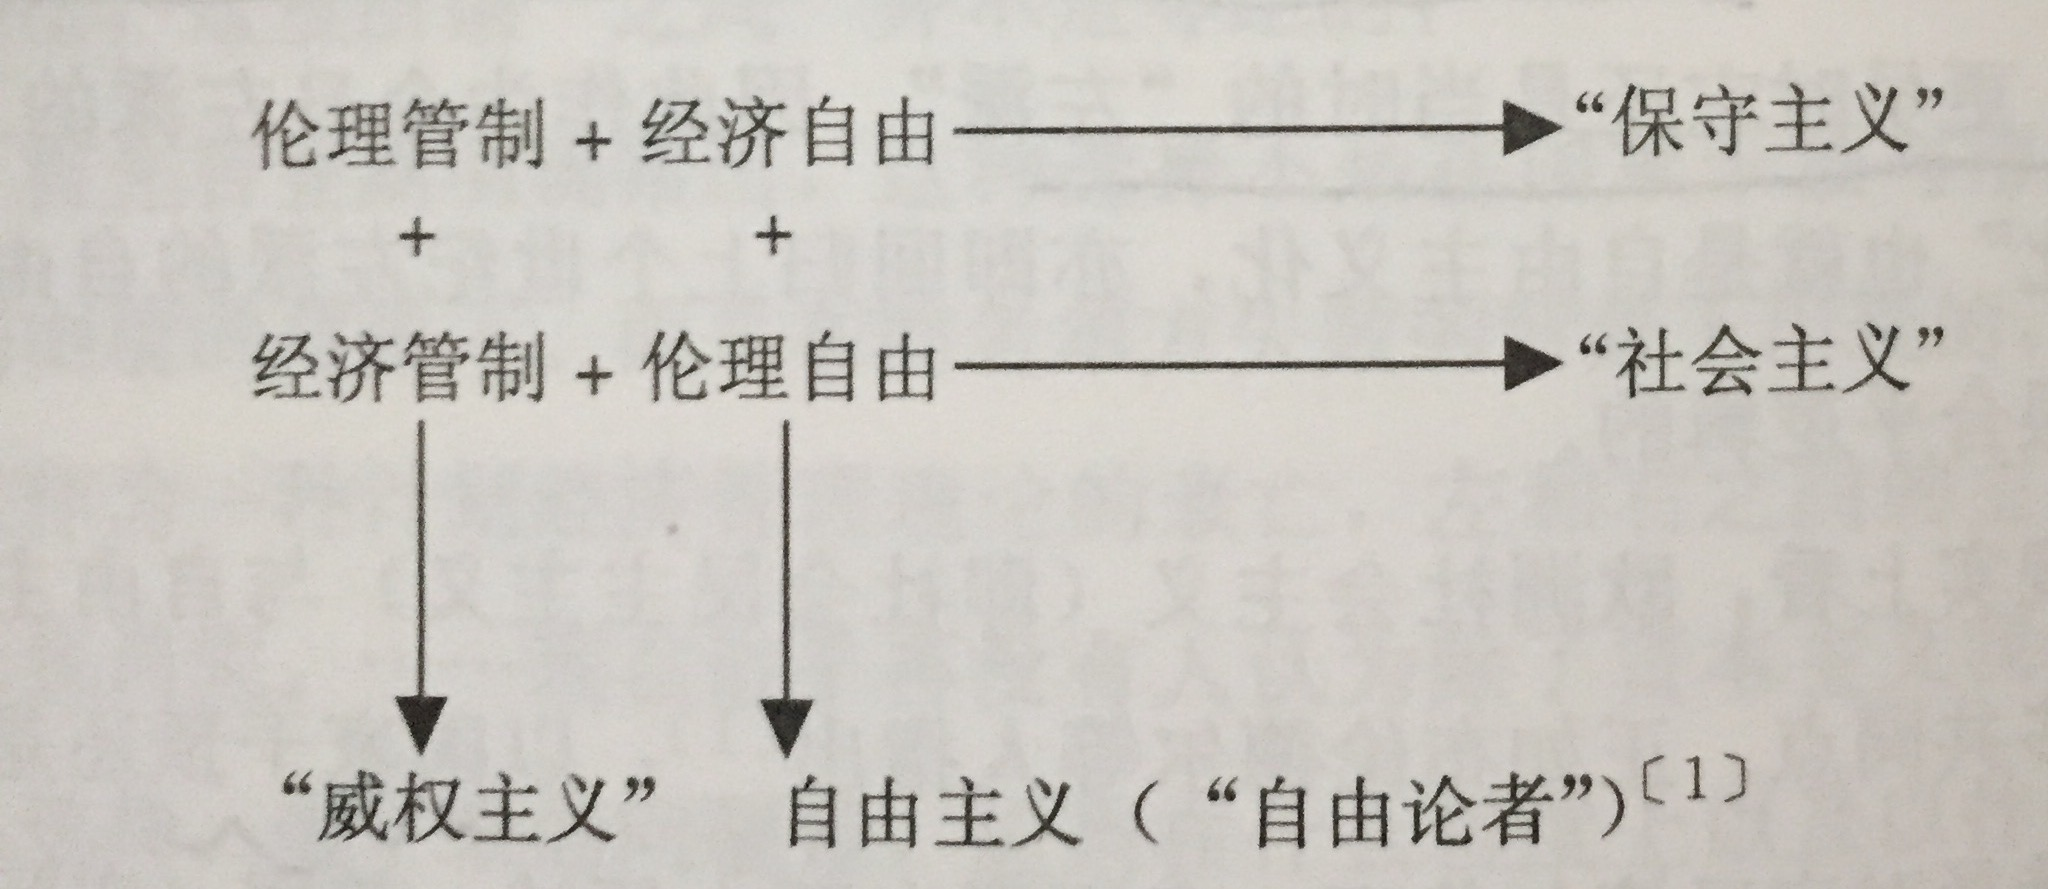
\includegraphics[width=0.5\linewidth]{images/zhuyi2.jpg}
\end{figure}

秦晖是自由主义者,认为自由主义“一个基本内容就是强调‘群己权界’。公域讲民主,私域讲自由”。

宪政的目的就是要使政府的权力与责任相对应,这种权力必须为被统治者所授予,而授予的唯一目的就是要政府能够向被统治者负责。宪政与民主是两回事,前者追求权责对应,后者追求多数决定。前者讲的是权力运用的规则,后者讲的是权力的来源。无民主则宪政原则不能贯彻到底,无宪政则民主机制更会走向反面。 
\begin{figure}[htpb]
\centering
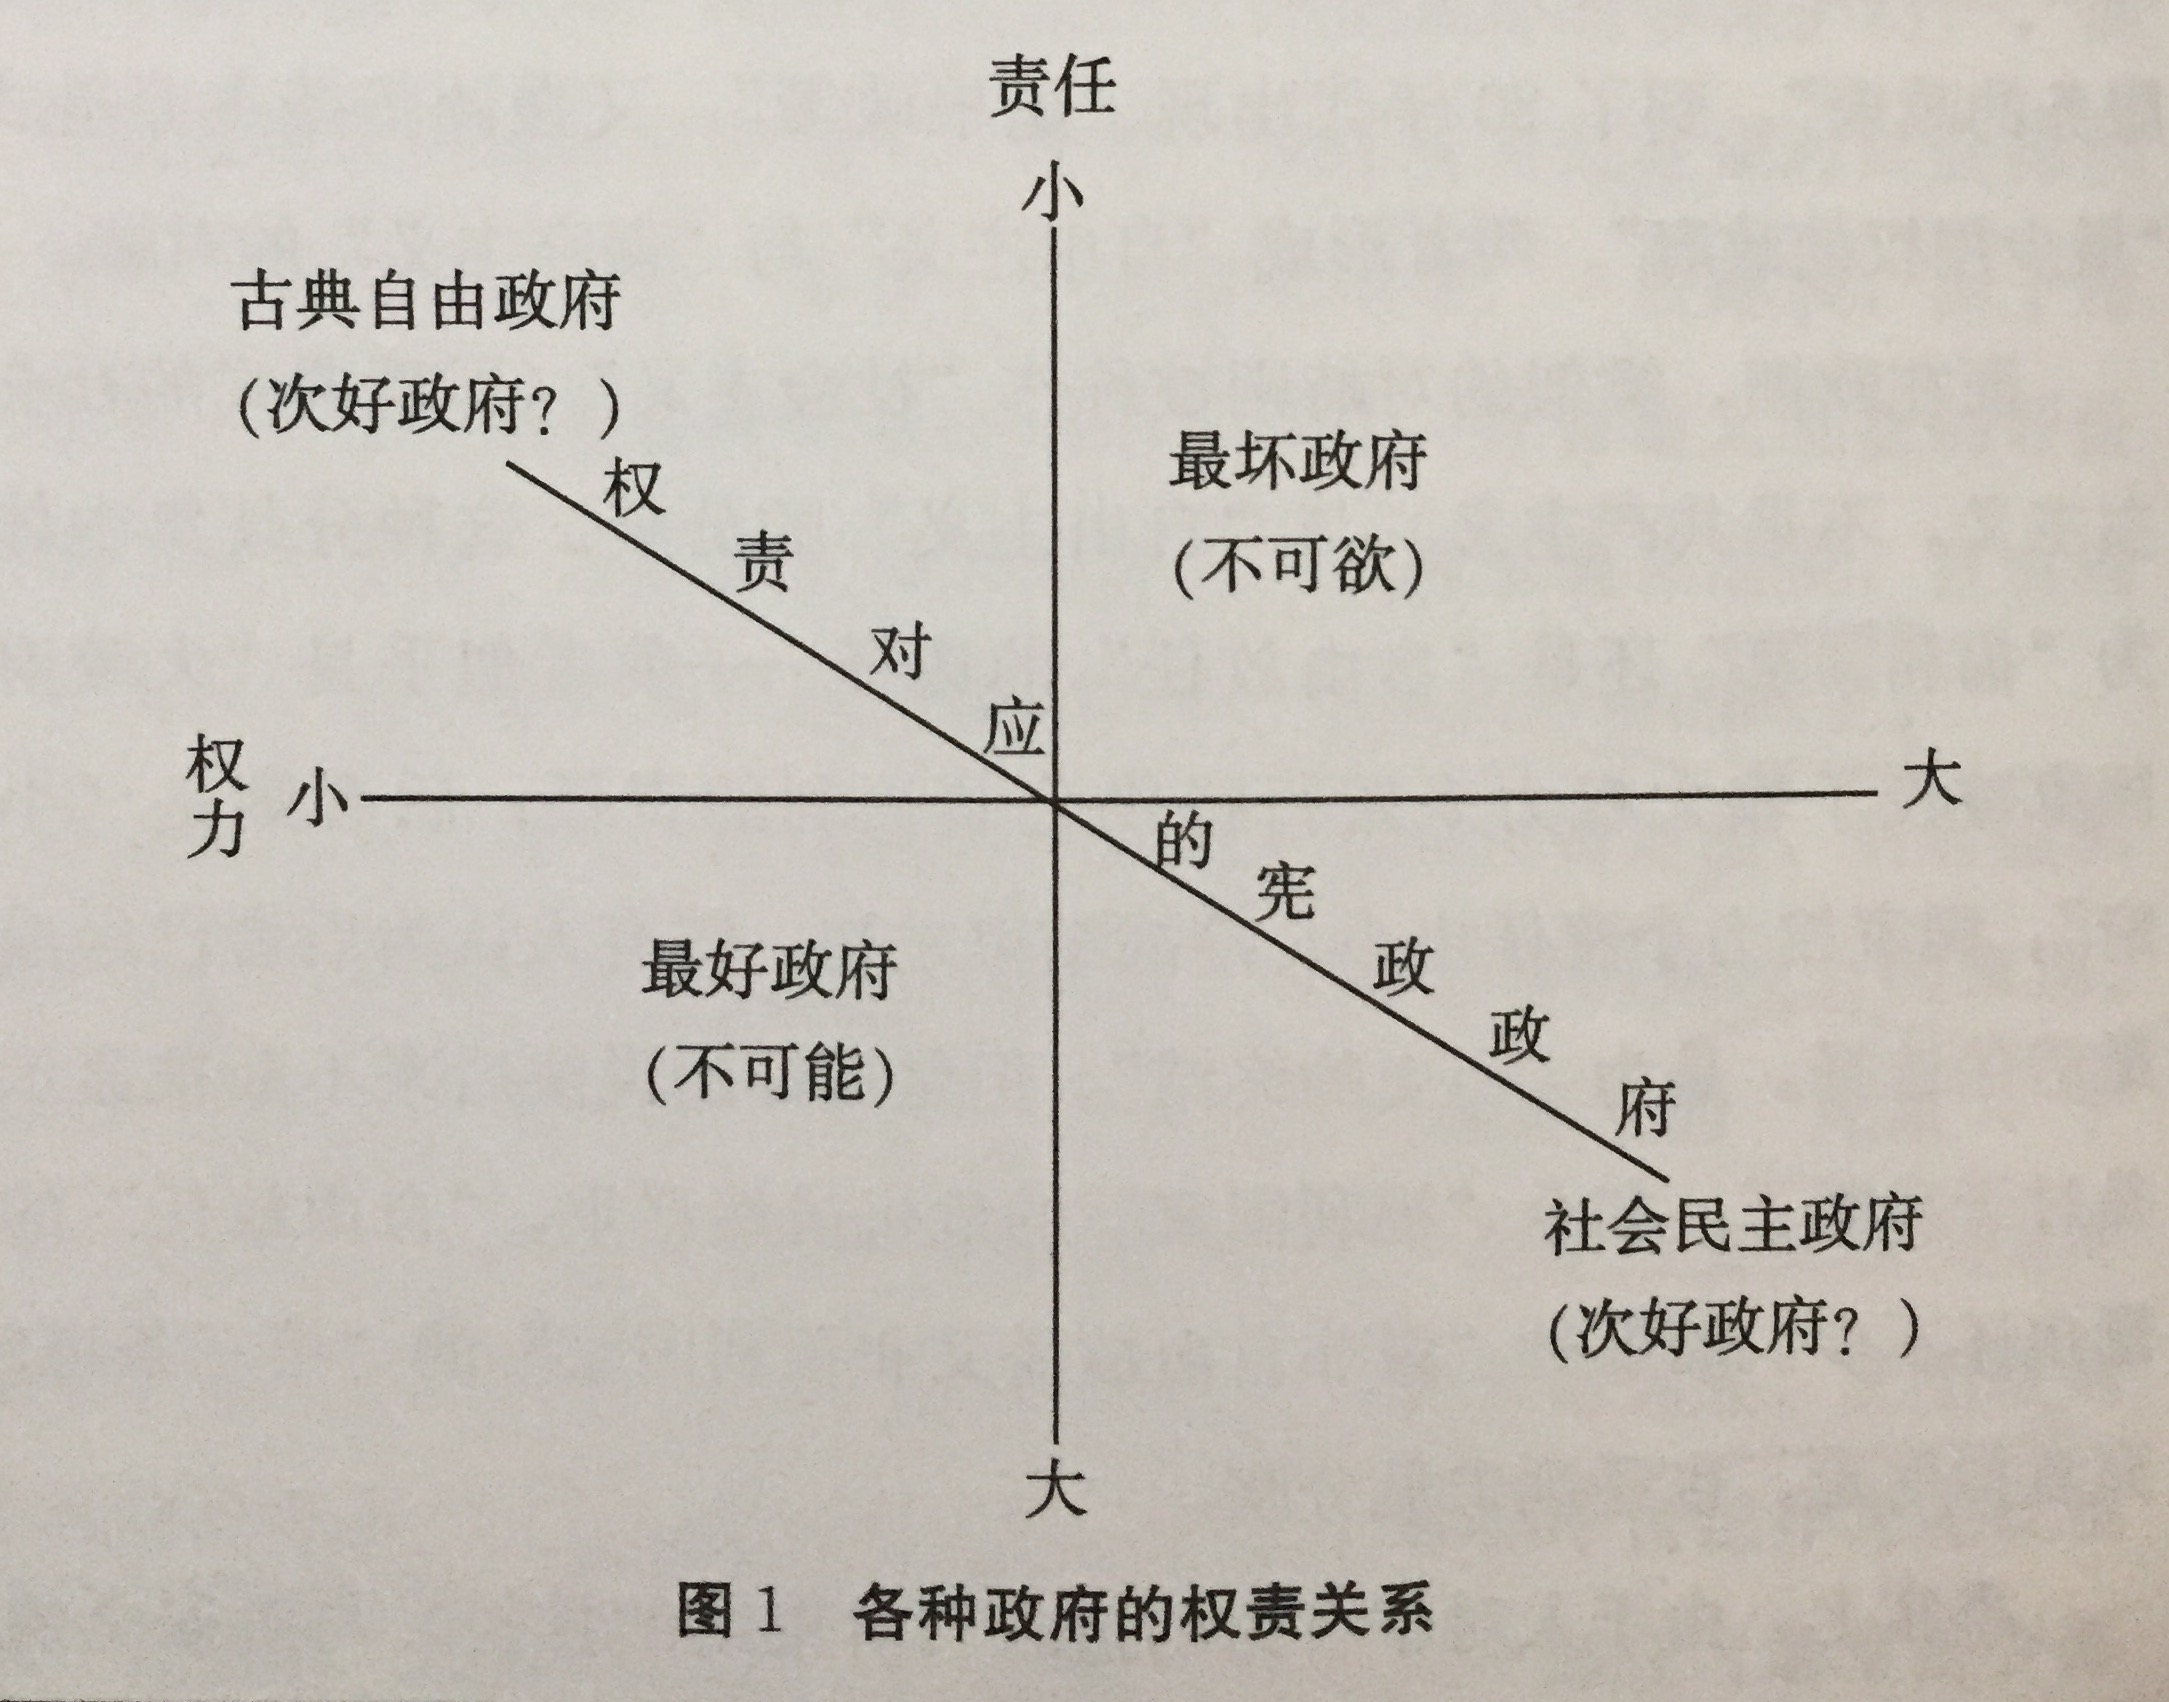
\includegraphics[width=0.5\linewidth]{images/zhengfu.jpg}
\end{figure}

为了捍卫公正,哈耶克主张可以引申为\emph{过程公正,既往不咎},诺齐克主张\emph{过程公正必咎既往,原则上可以一直追溯到”最初获得“}。

\subsubsection{关于俄国革命}
俄国十九世纪末二十世纪初的改革和随后而来的革命是中国革命的样板。这段时间内:
\begin{quotation}
俄国民粹派一方面极言知识分子的虚伪、委琐与农民的朴实、崇高,甚至提出“知识分子应当拜倒在农民脚下”,但另一方面又强调束缚农民,所说农民一旦“脱离土地,忘记‘务农’,那么俄国人民、人民的世界观、人民发出的光和热便不复存在,剩下的只是空虚的灵魂、‘完全的自由自在’、可怕的‘爱上哪儿就上哪儿’”。
\end{quotation}
这是随后斯大林时代的文字注脚,同时被我党学过去,成为直至现在的文艺指导方针。

\subsubsection{关于中国的改革}